\chapter{The \alphat Analysis}
\label{ch:analysis}

% **************************** Define Graphics Path **************************
\ifpdf
    \graphicspath{{Chapter5/Figs/Raster/}{Chapter5/Figs/PDF/}{Chapter5/Figs/}}
\else
    \graphicspath{{Chapter5/Figs/Vector/}{Chapter5/Figs/}}
\fi


%********************************** % First Section  *************************************
\section{Analysis Overview}  %Section - 1.1 
\label{sec:selection_analysis_overview}

Analyses searching in the jets and \met final state encounter significant 
backgrounds from SM sources of both genuine and fake \met. Genuine \met 
originates from \ttbar, W and Z boson production, with one or more
neutrinos in the final state. In this analysis background predictions are made
for these processes using 
extrapolations into the signal region from independent, process-specific control
samples, as described in Chapter~\ref{ch:background}.
Fake \met predominantly originates from mismeasurement of QCD 
multijet (MJ) production, which is the dominant process in the hadronic
environment
and  phase space considered in this analysis due to its very large cross
section.  Small inconsistencies in the handling of such large backgrounds or
rare detector effects can therefore 
have a significant impact on an analysis. This background is reduced to an 
entirely negligible level using the dimensionless kinematic variable \alphat.

% OLD
% Analyses searching in the jets and \met final state encounter significant 
% backgrounds from SM sources of both genuine \met, originating from the leptonic 
% decays of W bosons, 
% and fake \met, originating from jet mismeasurement. The \alphat 
% analysis makes predictions for the former using a data-driven transfer factor 
% technique to extrapolate yields from statistically independent control samples 
% into the signal region. However the latter, sources of fake \met from QCD multijet events,
% are reduced to a negligible level using the kinematic 
% variable \alphat.

In this analysis, following the generic signal selection criteria (described in
Section~\ref{sec:selec_crit}), events are binned in exclusive categories of \HT, 
and the multiplicity of jets and b-tagged jets,  
\nj and \nb, as summarised in Table~\ref{tab:ht-bins}. Such binning allows for
targeted interpretations across the vast array of
possible simplified model final states, while reducing background yields to a 
minimum.

\begin{table}[ht!]
  \caption{\HT bin lower bounds used for each \nj and \nb category.\label
  {tab:ht-bins}}
  \centering
  \footnotesize
  \begin{tabular}{ lrrrrrrrrrrr }
    \hline
    \hline
    (\nj,\nb)       & \multicolumn{11}{c}{\HT bins (\gev)} \\
    \hline
    (2-3,0)           & 200 & 275 & 325 & 375 & 475 & 575 & 675 & 775 & 875 & 975 & $>$1075  \\
    (2-3,1)           & 200 & 275 & 325 & 375 & 475 & 575 & 675 & 775 & 875 & 975 & $>$1075  \\
    (2-3,2)           & 200 & 275 & 325 & 375 & 475 & 575 & 675 & 775 & $>$875   & \multicolumn{2}{c}{} \\
%    (2-3,3)          & 200 & 275 & 325 & 375 & 475 & 575 & 675 & 775 & $>$875   & \multicolumn{2}{c}{} \\
    ($\geq$4,0)       & 200 & 275 & 325 & 375 & 475 & 575 & 675 & 775 & 875 & 975 & $>$1075  \\
    ($\geq$4,1)       & 200 & 275 & 325 & 375 & 475 & 575 & 675 & 775 & 875 & 975 & $>$1075  \\
    ($\geq$4,2)       & 200 & 275 & 325 & 375 & 475 & 575 & 675 & 775 & $>$875   & \multicolumn{2}{c}{} \\
    ($\geq$4,3)       & 200 & 275 & 325 & 375 & 475 & 575 & 675 & 775 & $>$875   & \multicolumn{2}{c}{} \\
    ($\geq$4,$\geq$4) & 200 & 275 & 325 & $>$375   & \multicolumn{7}{c}{}    \\
    \hline
    \hline
  \end{tabular}
\end{table}

The main analysis search region is described in the remainder of this chapter.


\subsection{The \alphat kinematic variable}
\label{sec:alphat}

% QCD multijet (MJ) events dominate the SM background in any search with multiple jets 
% in the final state. Jet energy mismeasurements in a 
% purely QCD MJ event can lead to non-negligible amounts of \mht, therefore 
% passing the signal selection.
Attempting to accurately measure the QCD contribution to the total background is
particularly challenging given the hadronic environment of the LHC and the lack
of precise measurements and calculations of the large multijet cross sections
involved. As an
alternative approach, the goal of this analysis is to reduce QCD down to
entirely negligible levels with respect to background processes with genuine
\met, achieved through the use of the dimensionless kinematic
variable, \alphat. The di-jet variable
$\alpha$ was first proposed by Randall et al.\ in 2008~\cite{Randall:2008rw},
and later translated into the transverse plane for use with LHC
analyses~\cite{CMS:2008vya, CMS-PAS-SUS-09-001}.
\alphat is defined for di-jets as:
% 
\begin{equation}
\alphat = \frac{ \sqrt{E_T^{j_2}/E_T^{j_1}} }{ \sqrt{2(1-cos(\Delta \phi))} } ,
\label{eq:alphat_di-jet}
\end{equation}
% 
where $E_T^{j_1}$ and $E_T^{j_2}$ are the reconstructed transverse energies of 
the first and second \Pt-ordered jets respectively, and $\Delta \phi$ is the separation 
between the two jets in the $\phi$ plane.

A perfectly measured di-jet event containing back to back jets in $\phi$ of equal energy will
have an \alphat value of 0.5, whereas 
events with \met originating from jet energy mismeasurements will have values of $\alphat<0.5$.
Only events containing sources of genuine \met, whether from SM or BSM sources,
can have values of $\alphat > 0.5$.
% 
% \begin{equation}
% \alphat = \frac{E_T^{j_2}}{M_T} = \frac{\sqrt{}}
% \label{eq:alphat_di-jet}
% \end{equation}
% 
% where $E_T^{j_2}$ is the transverse energy of the less energetic jet and $M_T$ 
% is the transverse mass of the di-jet system, defined as:
% 
% \begin{equation}
% M_T = \sqrt{\bigg(\sum^2_{i=1}{E_T^{j_i}}\bigg)^2 - \bigg(\sum^2_{i=1}{p_x^{j_i}}\bigg)^2 - \bigg(\sum^2_{i=1}{p_y^{j_i}}\bigg)^2}
% \label{eq:mt}
% \end{equation}
% 
% where $E_T^{j_i}$, $p_x^{j_i}$ and $p_y^{j_i}$ are the transverse energy and 
% transverse momentum in the $x$ and $y$ planes, for the jet $j_i$.

% The \alphat variable can be generalised to an n-jet case by considering the event as a 
% pseudo-di-jet system, constructing each pseudo-jet such that the difference in \HT
% between each pseudo-jet system, \deltaHT, is minimised. \alphat then takes the 
% form:
The \alphat variable can be generalised to any higher jet multiplicity by reducing an n-jet
system to two pseudo-jets. Each pseudo-jet is constructed from any number of jets.
All possible combinations are considered with the goal of finding the configuration
for which the difference in \HT between each pseudo-jet, \deltaHT, is minimised.
\alphat then takes the form:

% 
\begin{equation}
\alphat = \frac{1}{2} \times \frac{\HT-\deltaHT}{\sqrt{\HT^2 - \mht^2}} = 
\frac{1}{2} \times \frac{1-\frac{\deltaHT}{\HT}}{\sqrt{1 - \big(\frac{\mht}
{\HT}\big)^2}}.
\label{eq:alphat_njet}
\end{equation}
% 

The \alphat variable leads to a correlation between the two variables of \mht
and \deltaHT, as demonstrated in Figure~\ref{fig:alphat_corr} by the black contours of
constant \alphat. 
As QCD events (Figure~\ref{fig:alphat_corr_qcd}) contain no genuine source of missing
energy they exhibit a correlation between the two variables \mht and \deltaHT. 
%
\begin{figure}[b!]
  \centering
  \begin{subfigure}[t]{.46\textwidth}
    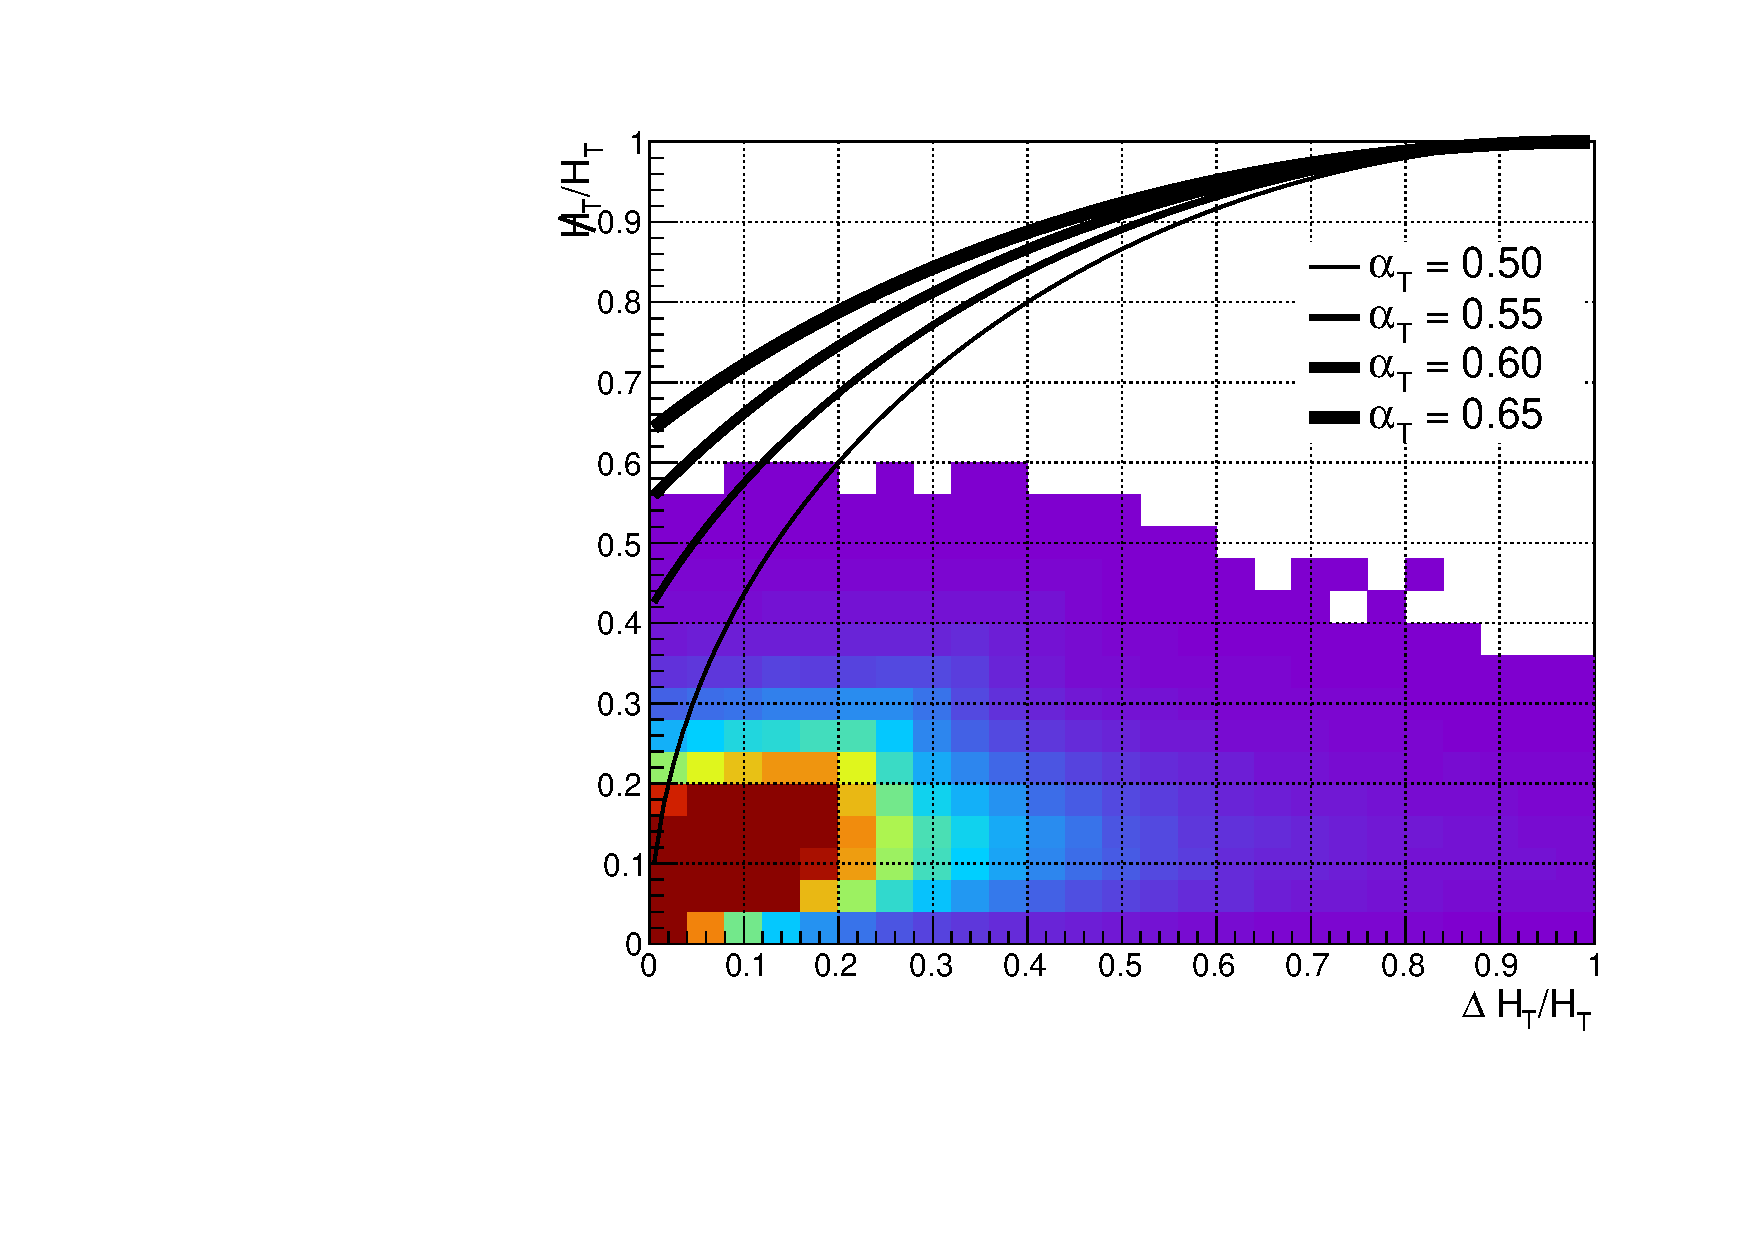
\includegraphics[width=\textwidth]{Figs/alphat/alphat_correlation_QCD_ge4j_done3.pdf}
    \caption{QCD}
    \label{fig:alphat_corr_qcd}
  \end{subfigure}
  \begin{subfigure}[t]{.46\textwidth}
    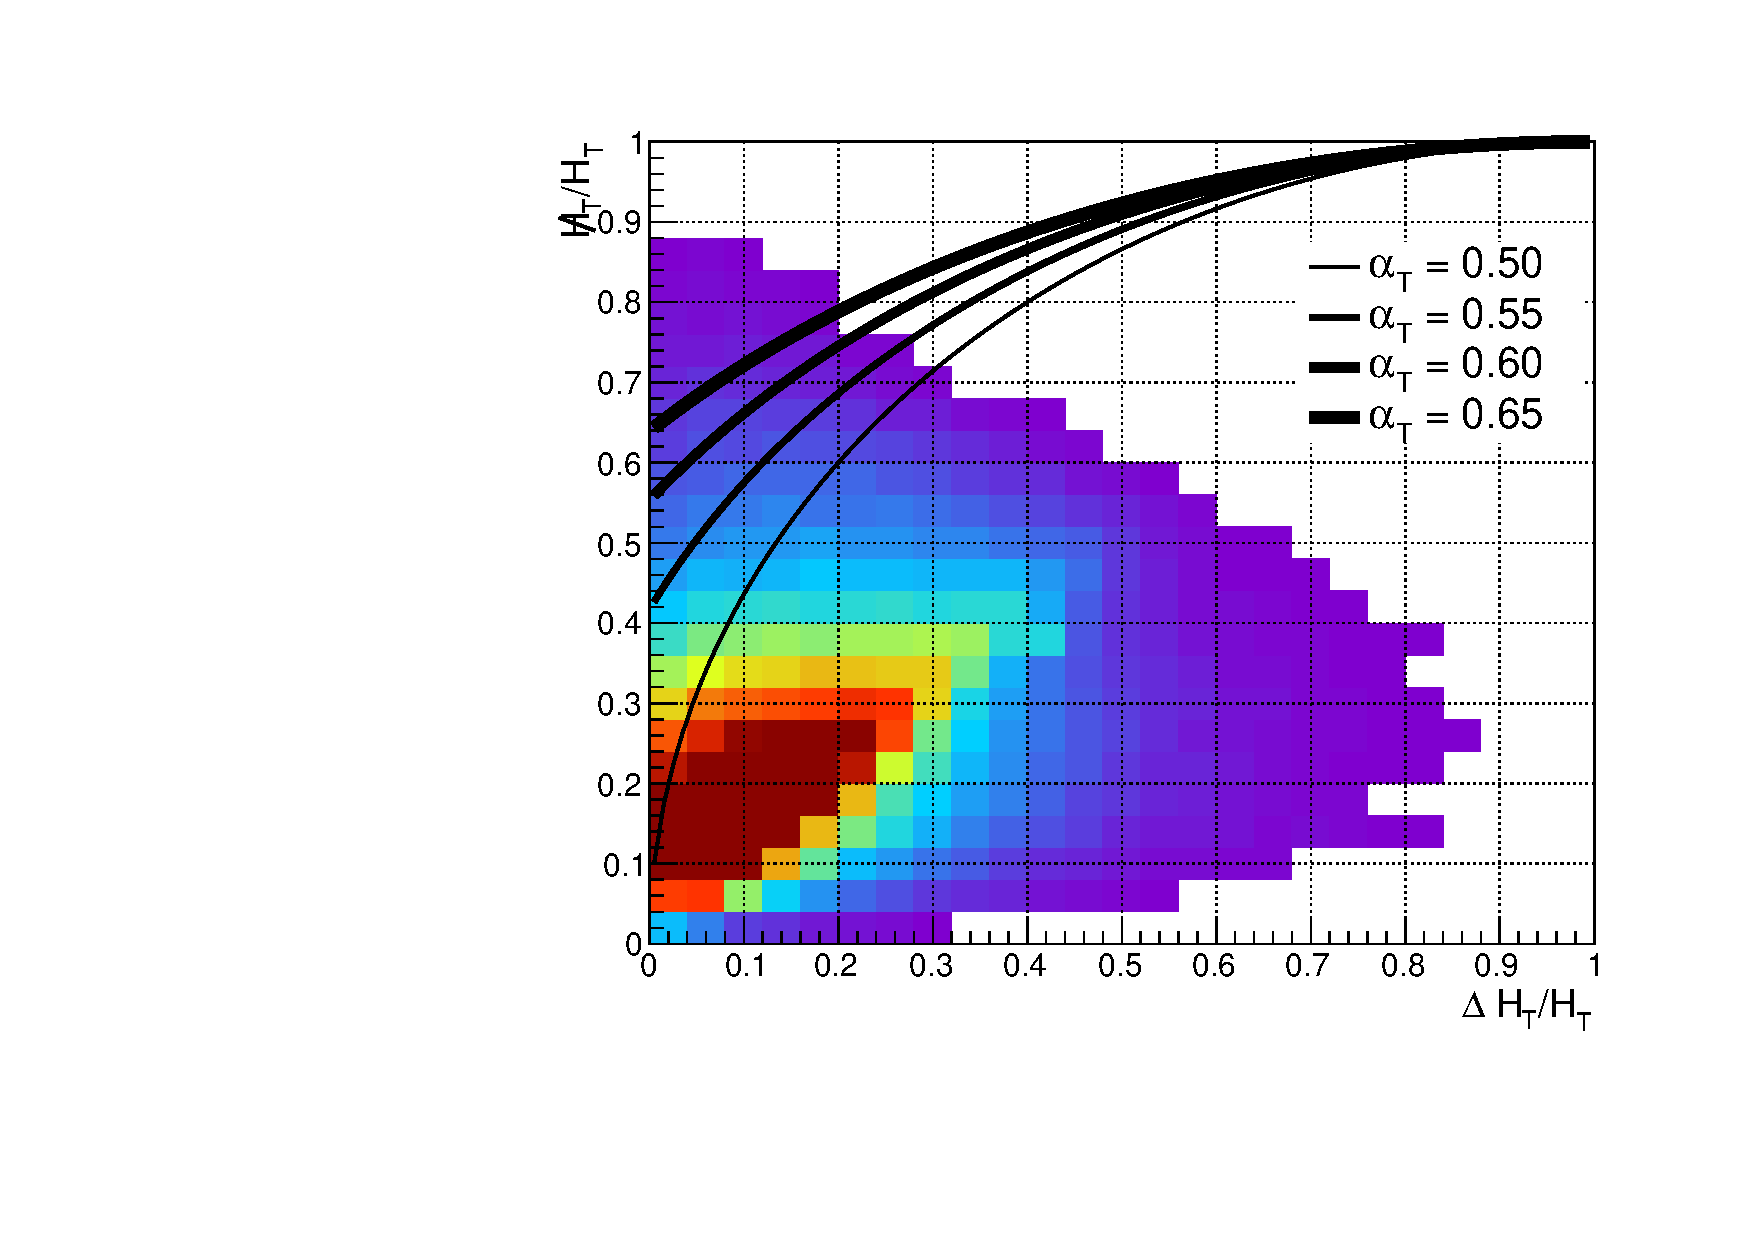
\includegraphics[width=\textwidth]{Figs/alphat/alphat_correlation_Zinv_ge4j_done3.pdf}
    \caption{\zinv}
    \label{fig:alphat_corr_zinv}
  \end{subfigure}\\
  \begin{subfigure}[t]{.46\textwidth}
    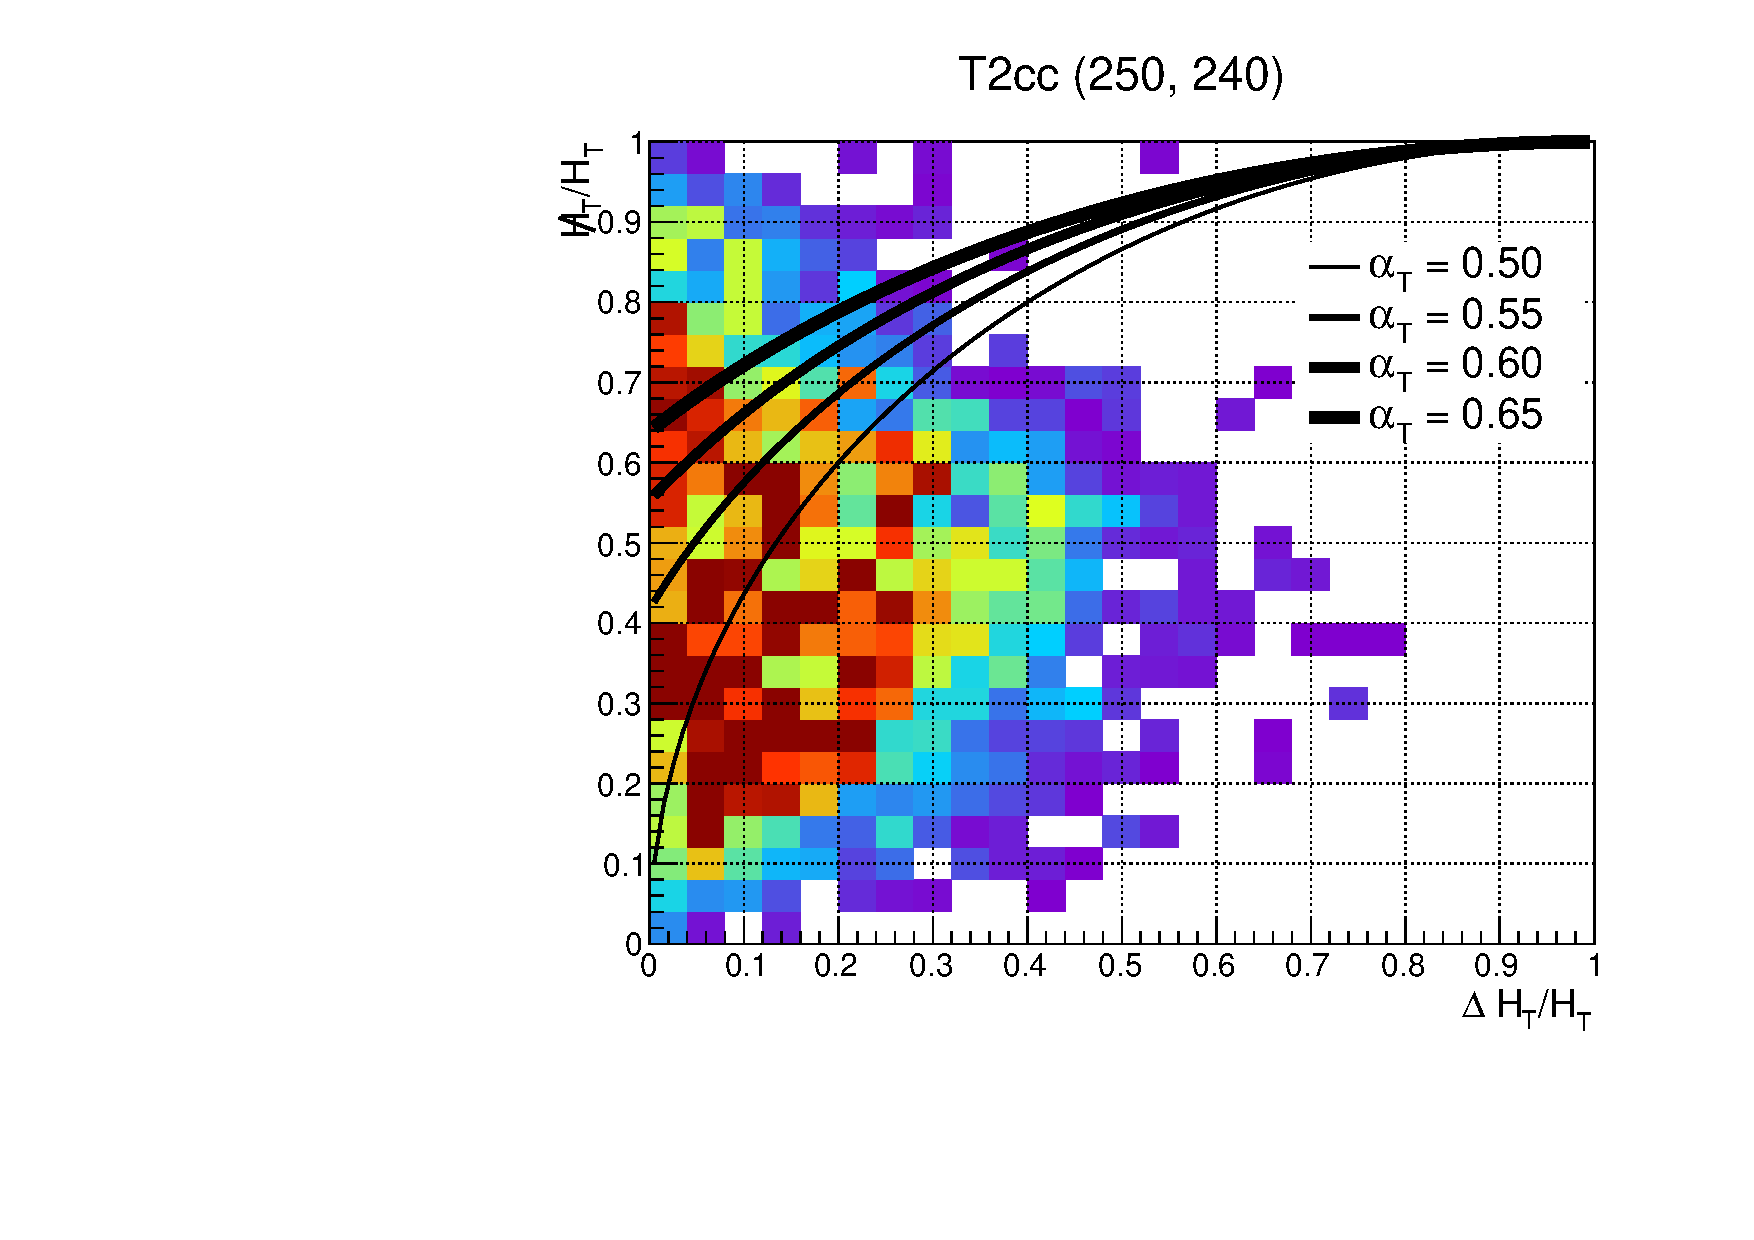
\includegraphics[width=\textwidth]
    {Figs/alphat/alphat_correlation_T2cc_250_240_ge4j_done3.pdf}
    \caption{Charm decay model (250, 240)}
    \label{fig:alphat_corr_t2cc}
  \end{subfigure}
  \caption{The correlation between \mht and \deltaHT for MC samples of QCD,
  \zinv and an example mass point of the charm decay signal model ($m_{\sTop} =
  250$~\gev, $m_{\chiz} = 240$~\gev). Contours of constant \alphat are shown in
  black. Each axis is normalised according to the event \HT.}
  \label{fig:alphat_corr}
\end{figure}
%
They
sit at low \mht, where missing energy arises predominantly due to jet
mismeasurement, thereby largely having \alphat < 0.5. Invisible decays of the Z-boson
(Figure~\ref{fig:alphat_corr_zinv}) sit at higher values of \mht due to the
presence of neutrinos in the final state, allowing them to achieve \alphat values
greater than 0.5. Finally a SUSY decay (Figure~\ref{fig:alphat_corr_t2cc}), with
genuine missing transverse energy provided by the neutralino, breaks any correlation
between \mht and \deltaHT, sitting also at higher values of \alphat.


Through the requirement of \alphat in a given region of \HT, a certain missing
energy threshold is implied. Figure~\ref{fig:alphat_mht_corr} shows this
relationship for
the assumption of \deltaHT = 0 - an assumption which yields the minimum \mht
values. Given this correlation, the implicit missing energy threshold can be
maintained across the \HT range by lowering the \alphat thresholds in the high
\HT
region.

\begin{figure}
  \centering
  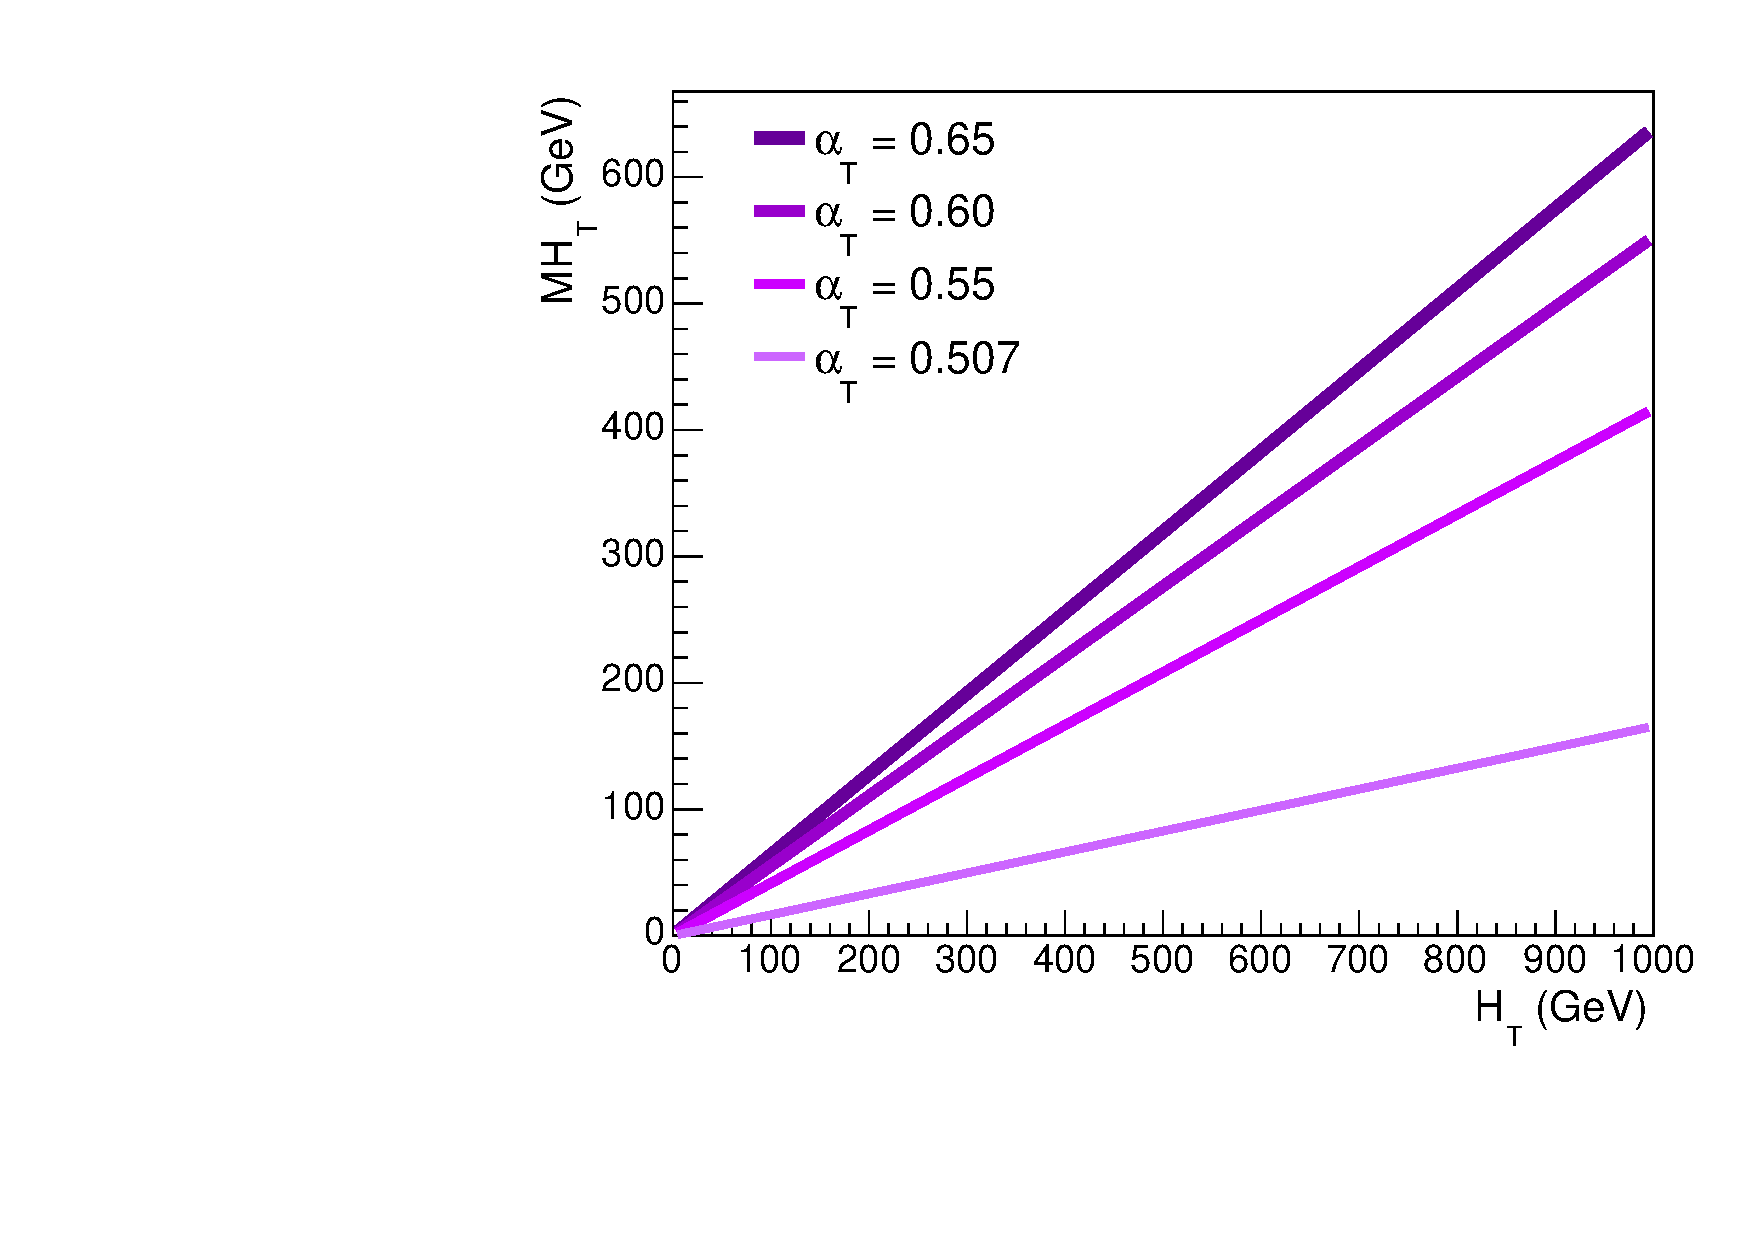
\includegraphics[width=0.7\textwidth]{Figs/alphat/mht_correlation.pdf}
  \caption{The correlation between \HT and \mht for different \alphat values,
  with the assumption of \deltaHT = 0.}
  \label{fig:alphat_mht_corr}
\end{figure}

%********************************** % First Section  *************************************

\section{Standard Model Backgrounds}
\subsection{Genuine \met}
The dominant Electroweak (EWK) source of genuine missing energy comes from
Z-boson production where the Z decays
to neutrinos, \zinv, with associated jets. This source of background
is considered irreducible.

Events containing leptonic decays of W bosons, \wlnu, originating either
from direct W production, or via the decay of a top quark from \ttbar 
production, are sources of genuine 
missing energy due to the presence of a weakly interacting neutrino which
evades detection. Such events are vetoed in the signal
region due to the presence of a 
lepton. However, if the lepton is not detected, leptonic W decays 
can pass the signal selection, forming a significant SM background.

% While lepton and photon vetoes employed in the signal region suppress 
% significant amounts of background from events with neutrinos, such events can 
% still persist if, for example, the lepton is not identified.
% Such processes are predominantly from \ttbar or W-boson production, where the 
% W decays via \wlnu. If the lepton is `lost' and evades our 
% lepton vetoes, significant missing energy can be produced not only from missing 
% the lepton, but from the presence of the neutrino. When such processes are accompanied 
% by associated jet production they are then able to pass our signal region selection.

Leptons can be `lost' for a variety different reasons, but ultimately for failing
the lepton ID criteria. There are numerous potential causes, the 
most prevalent being soft-leptons below the ID's \Pt threshold or non-isolated
leptons
which pass the ID quality cuts but fail the isolation requirement.


% \emph{move to selection section}
% Events containing a Single Isolated Track (SIT) are vetoed from the signal 
% region. This tracker based veto is particularly useful for vetoing additional events 
% that contain leptons which have failed our lepton ID requirements entirely, and 
% are therefore not considered by the leptonic vetoes. Additionally, the veto also
% removes background contributions from single-pronged hadronic decays of $\tau$
% leptons.

% While originally designed to target hadronically decaying tau leptons, 
% this requirement reduces the remaining lost-lepton backgrounds also.

Following the hadronic selection requirements (outlined in
Section~\ref{sec:selec_crit}),
any remaining contributions from SM EWK backgrounds are estimated using a 
fully data-driven transfer factor technique, described in detail in
Section~\ref{sec:background_overview}.

\subsection{Fake \met}

As mentioned previously, the dominant source of background for analyses 
searching for a multijet final state is from QCD. A fully-measured QCD event 
would consist of multiple jets balancing each other in all planes. However, in 
order to enter the signal region an event must contain missing energy, 
\mht (equivalent to \met in all-hadronic events).

The most common way for a balanced multijet (MJ) event to gain \mht occurs if
one
or more of the jets are mismeasured, such that their vectorial sum leads to non-zero
\mht. This can occur due to detector issues, or due to stochastic fluctuations
within the inherent jet-resolution of the 
detector. The former is protected against by the \met filters summarised in 
Table~\ref{tab:met_filters} and using a further filter to remove events
affected by non-functioning or damaged regions of the ECAL system, where 
events are vetoed if they contain significant energy deposits within a given 
distance from a known problematic region. The latter is dealt with using a
cut on the \alphat variable where 
events with fake missing energy signatures give values $<0.5$.

QCD MJ events can also appear to contain non-zero missing energy 
due to the threshold requirements of jets. If an event contains 
one or more jets below the analysis threshold, then the 
event is measured as imbalanced and containing \mht. Events such as these are largely 
removed with the \alphat requirement, however in addition a requirement is made on the
ratio \mhtmet.

Details of residual QCD cleaning cuts are given later in
Section~\ref{sec:qcd_cleaning}.

% Finally, it is also possible for rare instrumentation effects to lead to jet 
% energy
% mismeasurements. To protect against this, a suite of MET filters are defined by 
% the JetMET \emph{POG}, and are applied to all selections.


\section{Signal Triggers}
\label{sec:signal_triggers}

Events are collected at the HLT using a dedicated suite of
signal triggers. For an event to pass the trigger
requirements, it must exceed both a \HT and an \alphat threshold. Trigger rate 
can be maintained by varying the
threshold on each of these independent requirements, as shown in
Table~\ref{tab:sig_trigs}. Each \HT bin in the analysis is seeded by a
specific signal
trigger, with a 25~\gev offset between online \HT threshold used in the trigger itself
and offline \HT threshold used to define the \HT bin (with the
exception of the 200~\gev bin, for which the two thresholds are equal).

Exclusively for this analysis, the additional `Parked' trigger 
\\\verb!HT200_AlphaT0p57! is included, seeding the new \HT> 200~\gev bin. Such a low
threshold allows sensitivity to be maintained for softer physics signatures, such
as those expected from compressed spectra SUSY decays studied in this work.

\begin{table}[!b]
  \caption{Signal triggers, the L1 seed triggers and their efficiencies measured
  for per \HT and \nj category.}
  \label{tab:sig_trigs}
  \centering
  \scriptsize
  \begin{tabular}{ cccccc }
    \hline
    \hline
    Offline \HT       & Offline \alphat & L1 seed (\verb!L1_?!)         & Trigger (\verb!HLT_?!)  & \multicolumn{2}{c}{Efficiency (\%)}          \\ [0.5ex]
    region (\gev)         & threshold       & (highest thresholds)          &                         & $2 \leq \nj \leq 3$ & $\nj \geq 4$       \\ [0.5ex]
    \hline
    $200 < \HT < 275$ & 0.65            & \verb!DoubleJetC64!           & \verb!HT200_AlphaT0p57! & $81.8^{+0.4}_{-0.4}$  & $78.9^{+0.3}_{-0.4}$ \\
    $275 < \HT < 325$ & 0.60            & \verb!DoubleJetC64!           & \verb!HT200_AlphaT0p57! & $95.2^{+0.3}_{-0.4}$  & $90.0^{+1.2}_{-1.3}$ \\
    $325 < \HT < 375$ & 0.55            & \verb!DoubleJetC64 OR HTT175! & \verb!HT300_AlphaT0p53! & $97.9^{+0.3}_{-0.3}$  & $95.6^{+0.9}_{-1.0}$ \\
    $375 < \HT < 475$ & 0.55            & \verb!DoubleJetC64 OR HTT175! & \verb!HT350_AlphaT0p52! & $99.2^{+0.2}_{-0.2}$  & $98.7^{+0.5}_{-0.7}$ \\
    $\HT > 475$       & 0.55            & \verb!DoubleJetC64 OR HTT175! & \verb!HT400_AlphaT0p51! & $99.8^{+0.1}_{-0.3}$  & $99.6^{+0.3}_{-0.7}$ \\
    \hline
    \hline
  \end{tabular}
\end{table}

Trigger efficiencies are measured using an unbiased single-muon reference
trigger,
\\\verb!HLT_IsoMu24_eta2p1!, via a muon tag and probe method where a
single-muon is selected and then subsequently ignored from the analysis when 
calculating event level variables such as \HT, \mht and \alphat. Efficiencies 
are measured for each \HT bin and for each \nj category, as summarised in 
Table~\ref{tab:sig_trigs}. Example trigger `turn-on' curves are shown for the 3 
lowest \HT bins in figures~\ref{fig:eff_alphat_le3j} and \ref{fig:eff_alphat_ge4j}.
The curves are shown both differentially and cumulatively, to show the
efficiency for events of a given \alphat value and above an \alphat threshold
respectively.
For the bins with \HT > 375~\gev, the triggers are measured as fully efficient.
Inefficiencies in the low \HT bins are
understood as being due to the relatively high threshold L1 seed trigger used
for this region, in order to maintain
low rates in the high PU environment encountered throughout \runone. Lower 
efficiencies are also observed in the \njhigh category due to the presence of 
softer jets, as an increased number of jets must equate to the same total \HT 
requirement of a given bin. A small number of events are found at values of
\alphat lower than the trigger threshold leading to spikes in the differential
turn-on curves at low \alphat values, and an efficiency pedestal in the
cumulative turn-on curves. Such
events originate from the difference between the online and offline calculations
of the \alphat variable, where some approximations are made online to reduce
latency in the trigger.

All triggers were present throughout \runone, however the 
\\\verb!HLT_HT200_AlphaT0p57! trigger was used as part of the `Parked' data
stream which was reconstructed at a later date, following the active data-taking
period. During data-taking triggers may have `prescale' factors applied to them 
such that only every $n$ triggered events are actually recorded. Crucially however,
the full suite of signal triggers remained without a prescale for the entirety of
the 8~\tev data-taking.

\clearpage
% \afterpage{%
\begin{figure}[p!]
  \centering
    \begin{subfigure}[b]{0.48\textwidth}
      
\includegraphics[width=\textwidth,page=11, trim=0 0 0 20, clip=true]{Figs/trigger/HT200_275_73_73_36_AlphaT_le3j_RunAtFNAL}
      \caption{Differential, $200 < \HT < 275 $~\gev}
    \end{subfigure}
    \begin{subfigure}[b]{0.48\textwidth}
      
\includegraphics[width=\textwidth,page=18, trim=0 0 0 20, clip=true]{Figs/trigger/HT200_275_73_73_36_AlphaT_le3j_RunAtFNAL}
      \caption{Cumulative, $200 < \HT < 275 $~\gev}
    \end{subfigure} \\
    \vspace{0.5cm}\begin{subfigure}[b]{0.48\textwidth}
      
\includegraphics[width=\textwidth,page=11, trim=0 0 0 20, clip=true]{Figs/trigger/HT275_325_73_73_36_AlphaT_le3j_RunAtFNAL}
      \caption{Differential, $275 < \HT < 325 $~\gev}
    \end{subfigure}
    \begin{subfigure}[b]{0.48\textwidth}
      
\includegraphics[width=\textwidth,page=18, trim=0 0 0 20, clip=true]{Figs/trigger/HT275_325_73_73_36_AlphaT_le3j_RunAtFNAL}
      \caption{Cumulative, $275 < \HT < 325 $~\gev}
    \end{subfigure} \\
    \vspace{0.5cm}\begin{subfigure}[b]{0.48\textwidth}
      
\includegraphics[width=\textwidth,page=11, trim=0 0 0 20, clip=true]{Figs/trigger/HT325_375_86_86_43_AlphaT_le3j_RunAtFNAL}
      \caption{Differential, $325 < \HT < 375 $~\gev}
    \end{subfigure}
    \begin{subfigure}[b]{0.48\textwidth}
      
\includegraphics[width=\textwidth,page=18, trim=0 0 0 20, clip=true]{Figs/trigger/HT325_375_86_86_43_AlphaT_le3j_RunAtFNAL}
      \caption{Cumulative, $325 < \HT < 375 $~\gev}
    \end{subfigure} \\
  
    \caption{\label{fig:eff_alphat_le3j}
      Differential (left) and cumulative (right) efficiency turn-on curves for 
      the signal triggers, for the three lowest \HT bins and \njlow.}
\end{figure}
\clearpage
% }

% \afterpage{%
\begin{figure}[p!]
  \centering
    \begin{subfigure}[b]{0.48\textwidth}
      
\includegraphics[width=\textwidth,page=11]{Figs/trigger/HT200_275_73_73_36_AlphaT_ge4j_RunAtFNAL}
      \caption{Differential, $200 < \HT < 275 $~\gev}
    \end{subfigure}
    \begin{subfigure}[b]{0.48\textwidth}
      
\includegraphics[width=\textwidth,page=18]{Figs/trigger/HT200_275_73_73_36_AlphaT_ge4j_RunAtFNAL}
      \caption{Cumulative, $200 < \HT < 275 $~\gev}
    \end{subfigure} \\
    \begin{subfigure}[b]{0.48\textwidth}
      
\includegraphics[width=\textwidth,page=11]{Figs/trigger/HT275_325_73_73_36_AlphaT_ge4j_RunAtFNAL}
      \caption{Differential, $275 < \HT < 325 $~\gev}
    \end{subfigure}
    \begin{subfigure}[b]{0.48\textwidth}
      
\includegraphics[width=\textwidth,page=18]{Figs/trigger/HT275_325_73_73_36_AlphaT_ge4j_RunAtFNAL}
      \caption{Cumulative, $275 < \HT < 325 $~\gev}
    \end{subfigure} \\
    \begin{subfigure}[b]{0.48\textwidth}
      
\includegraphics[width=\textwidth,page=11]{Figs/trigger/HT325_375_86_86_43_AlphaT_ge4j_RunAtFNAL}
      \caption{Differential, $325 < \HT < 375 $~\gev}
    \end{subfigure}
    \begin{subfigure}[b]{0.48\textwidth}
      
\includegraphics[width=\textwidth,page=18]{Figs/trigger/HT325_375_86_86_43_AlphaT_ge4j_RunAtFNAL}
      \caption{Cumulative, $325 < \HT < 375 $~\gev}
    \end{subfigure} \\
  
    \caption{\label{fig:eff_alphat_ge4j}
      Differential (left) and cumulative (right) efficiency turn-on curves for 
      the signal triggers, for the three lowest \HT bins and \njhigh.}
\end{figure}
\clearpage
% }


\section{Selection Criteria}
\label{sec:selec_crit}

Event selection requirements for the signal region are chosen with an
aim to
maintain sensitivity to hadronically decaying sparticle production, while 
rejecting as many QCD-type processes as possible. To do so, requirements are 
made on:

\begin{table}[b!]
  \caption{Jet \Et and \alphat thresholds per \HT bin.
  \label{tab:analysis_thresholds}}
  \centering
  \small
  \begin{tabular}{ lcccc }
    \hline
    \hline
    & \multicolumn{4}{c}{\HT bin} \\
    & 200--275 & 275--325 & 325--375 & $>$375 \\
    \hline
    Lead jet \Pt (\gev)       & 73.3     & 73.3     & 86.7     & 100.0  \\
    Second jet \Pt (\gev)     & 73.3     & 73.3     & 86.7     & 100.0  \\
    All other jets \Pt (\gev) & 36.7     & 36.7     & 43.3     & 50.0   \\
    \hline
    \alphat        & 0.65     & 0.60     & 0.55     & 0.55    \\
    \hline
    \hline
  \end{tabular}
\end{table}

% \begin{table}[b]
%   \caption{\alphat thresholds per \HT bin.\label{tab:alphat_thresholds}}
%   \centering
%   \footnotesize
%   \begin{tabular}{ lccc }
%     \hline
%     \hline
%     \HT bin        & 200--275 & 275--325 & $>$325 \\
%     \hline
%     Lead jet       & 0.65     & 0.60     & 0.55  \\
%     \hline
%     \hline
%   \end{tabular}
% \end{table}


\begin{description}
\item[Jets]
Events are required to contain at least two jets, and have
$\HT > 200$~\gev, to ensure the presence of significant hadronic activity.
They are categorised by \HT, with jet \Pt
requirements on the two leading and the remaining additional jets separately.
The jet \Pt thresholds vary as a function of the \HT bin of the event, as shown in
Table~\ref{tab:analysis_thresholds}, in order to maintain a similar kinematic
phase space throughout the \HT range. Additionally, the leading jet is required to be
in the barrel region of the calorimeter, $\eta_{lead-jet} < 2.5$.

\item[Leptons]
Any events containing leptons are vetoed to ensure only hadronic events
are considered, thereby suppressing events with genuine \met from leptonic decays to
neutrinos such as \wlnu. Furthermore, events are vetoed that contain a jet within
$\Delta R < 0.5$ of a muon which fails the ID criteria. 

\item[Photons]
Events containing photons are vetoed, for similar reasons as the leptonic 
vetoes, in order to maintain a purely hadronic environment.

\item[Single Isolated Tracks]
Events containing a Single Isolated Track (SIT) are vetoed from the signal 
region. This tracker based veto is particularly useful for vetoing additional events 
that contain leptons which have failed our lepton ID requirements entirely and 
are therefore not considered by the leptonic vetoes. Additionally, the veto also
removes background contributions from single-pronged hadronic decays of $\tau$
leptons.

\item[Event]
The topology of the event is required to pass a threshold of at least $\alphat >
0.55$, a requirement which itself varies as a function of the \HT category being
considered, chosen such that the signal triggers are in the efficiency
plateau, as summarised in Table~\ref{tab:analysis_thresholds}. While no
absolute \met requirement is made, the cut on
\alphat imposes an implied threshold, maintaining the analysis'
sensitivity to very low regions of \met as shown by Figure~\ref{fig:alphat_mht_corr}.
Furthermore, events are required to have
\mhtmet < 1.25 and \mindphistar > 0.3 (defined later in
Chapter~\ref{ch:background}).

\end{description}

A breakdown of the EWK background 
composition is shown in Figure~\ref{fig:background_decomp}, split into the main 
categories of \zinv, \wj, \ttbar and all remaining residual backgrounds, such as
single top quark, diboson and Drell-Yann processes.

\begin{figure}[hb!]
\centering
\hspace{0cm}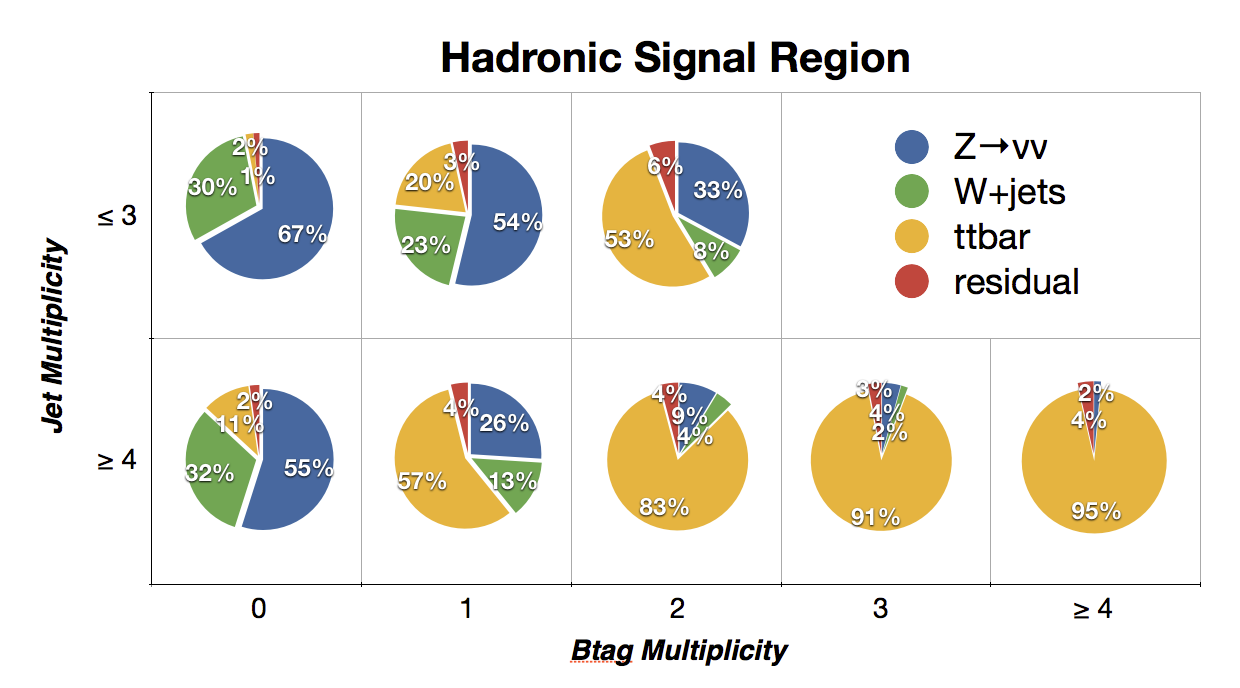
\includegraphics[width=0.9\textwidth, trim=0 00 0 0, clip=true]
{Figs/ra1_had_bg_comp_v3.png}
\caption{The breakdown of the total electroweak background into component
processes as a function of \nj and \nb, for \HT>200~\gev.}
\label{fig:background_decomp}
\end{figure}

\section{Example distributions and cutflow}

Example distributions of \alphat, \HT, \mht and jet \Pt  are
shown in Figure~\ref{fig:datamc_had_inc} for simulated SM processes,
following the full hadronic selection criteria, with an inclusive selection on \HT,
\nj and \nb. Even with this inclusive selection, \zinv is shown to be the biggest
contribution to the total SM background, with the `lost-lepton' sources of \wj and
\ttbar following. It is interesting to also note that \zinv and \wj have the hardest \mht
spectra, while \ttbar is softer. This is attributed to the greater probability of producing
back to back neutrinos, with their missing momenta contributions cancelling to give
lower \mht values.

Example cutflow yields are shown in
Table~\ref{tab:had_data_cutflow} for data in the \HT > 375~\gev region, employing
the full hadronic selection criteria, with an inclusive selection on \nj and \nb.
The cuts relate to those describe in this chapter, specifically in
Section~\ref{sec:selec_crit}. The requirement on \alphat is shown to reject many
orders of magnitude of events, as well as other `cleaning' cuts such as the deadECAL
filter and \mhtmet.

\begin{figure}[!ht]
  \centering
    \begin{subfigure}[b]{0.48\textwidth}
      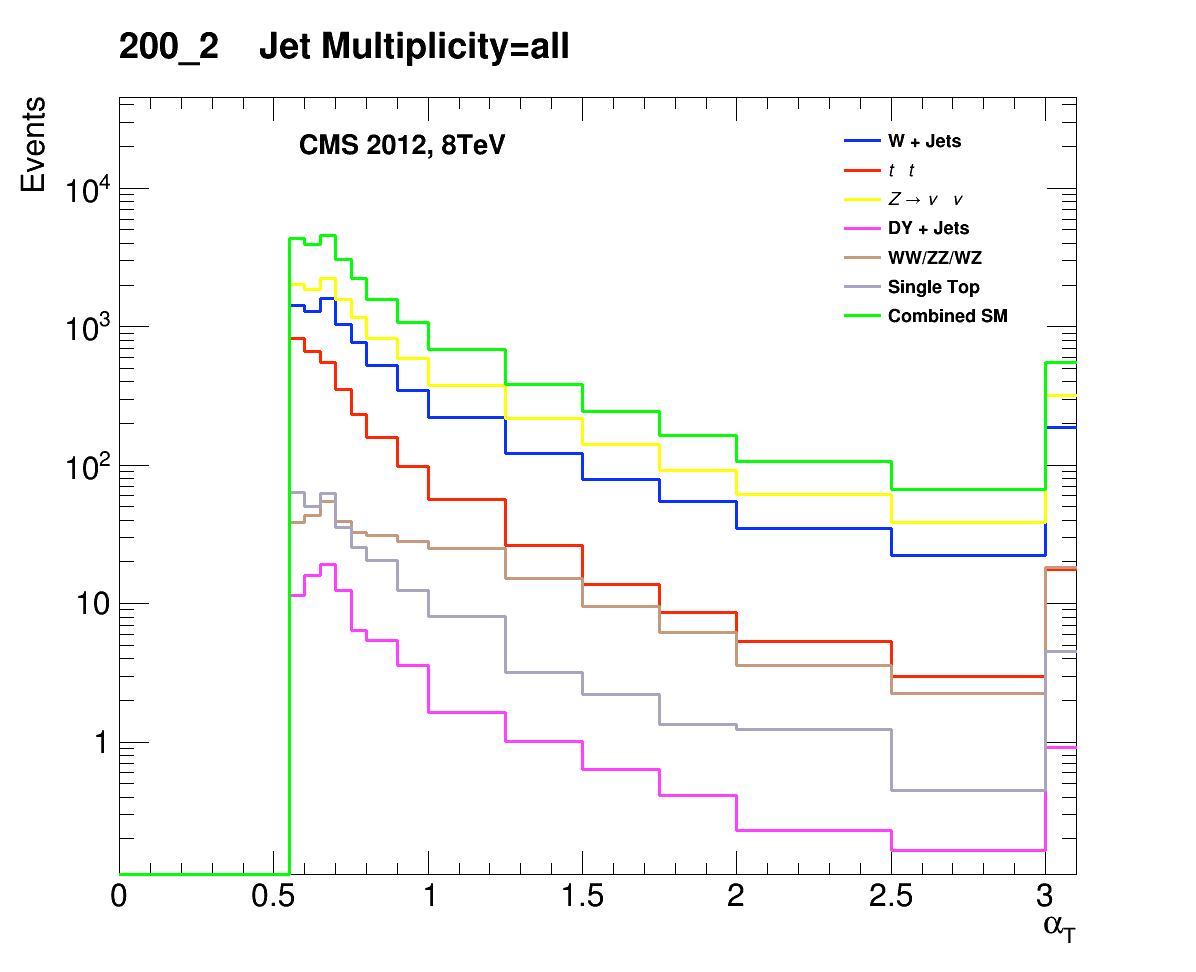
\includegraphics[width=\textwidth]{Figs/datamc/had/v1/AlphaT_all_200_upwards}
      \caption{\alphat}
    \end{subfigure}
    \begin{subfigure}[b]{0.48\textwidth}
      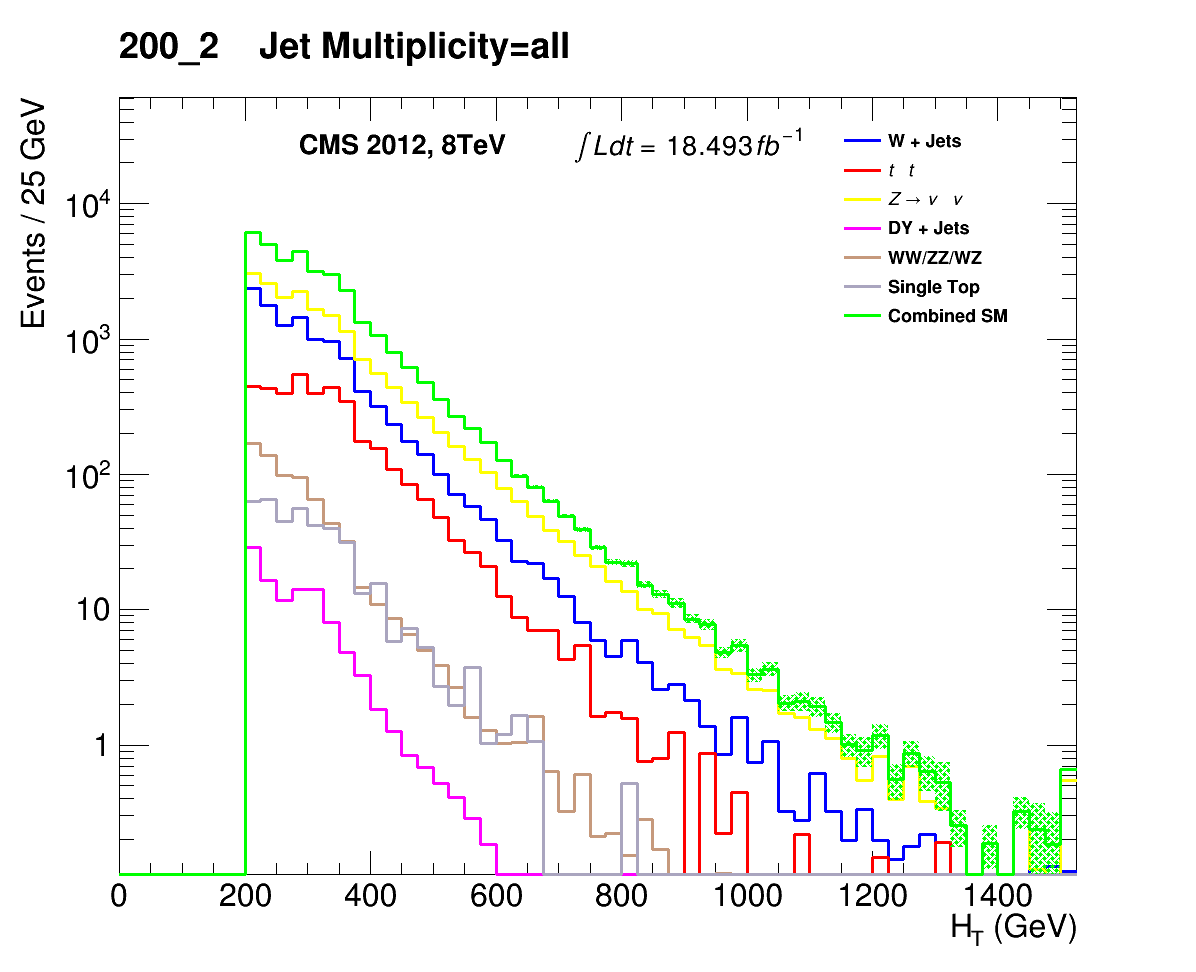
\includegraphics[width=\textwidth]{Figs/datamc/had/v1/HT_all_200_upwards}
      \caption{\HT}
    \end{subfigure} \\
    \begin{subfigure}[b]{0.48\textwidth}
      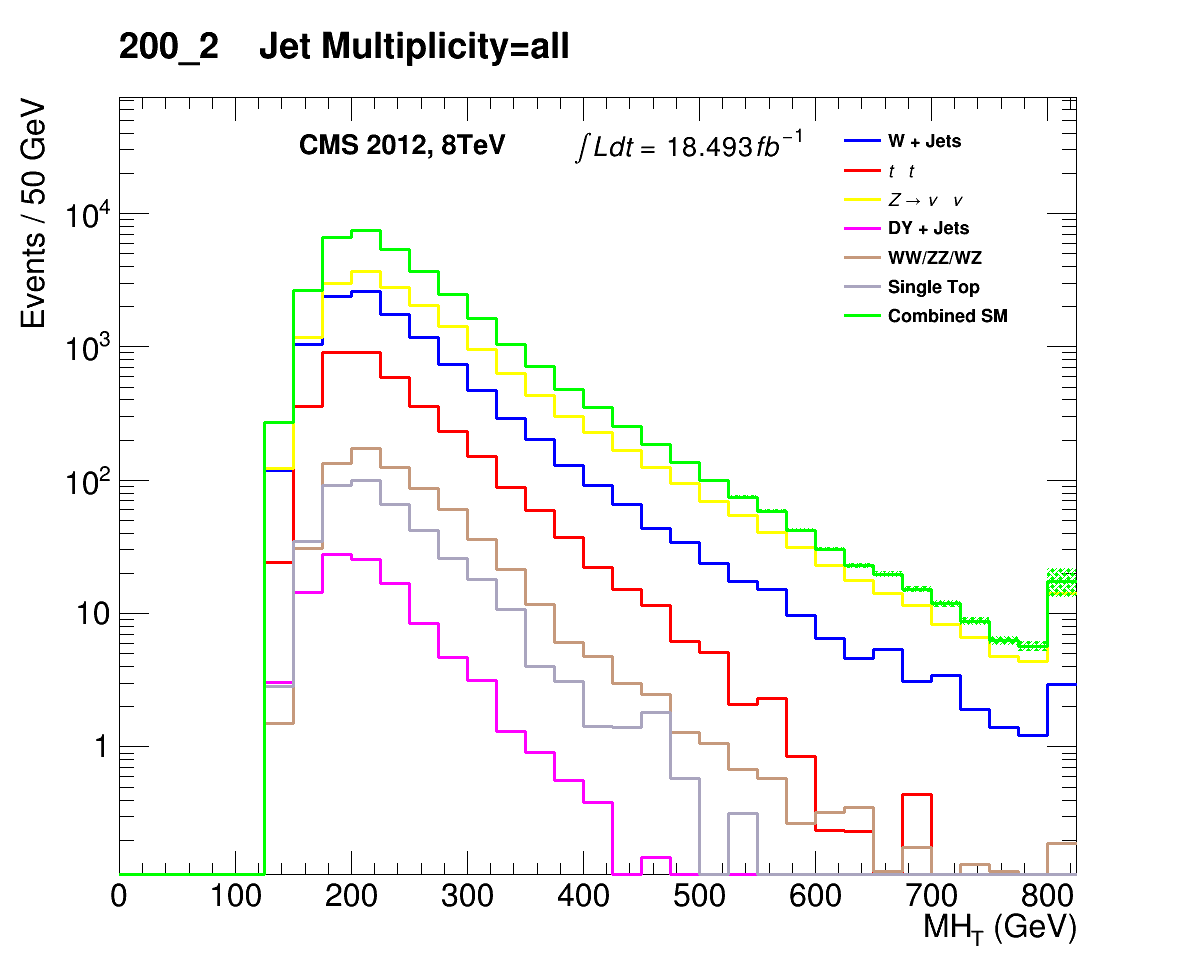
\includegraphics[width=\textwidth]{Figs/datamc/had/v1/MHT_all_200_upwards}
      \caption{\mht}
    \end{subfigure}
    \begin{subfigure}[b]{0.48\textwidth}
      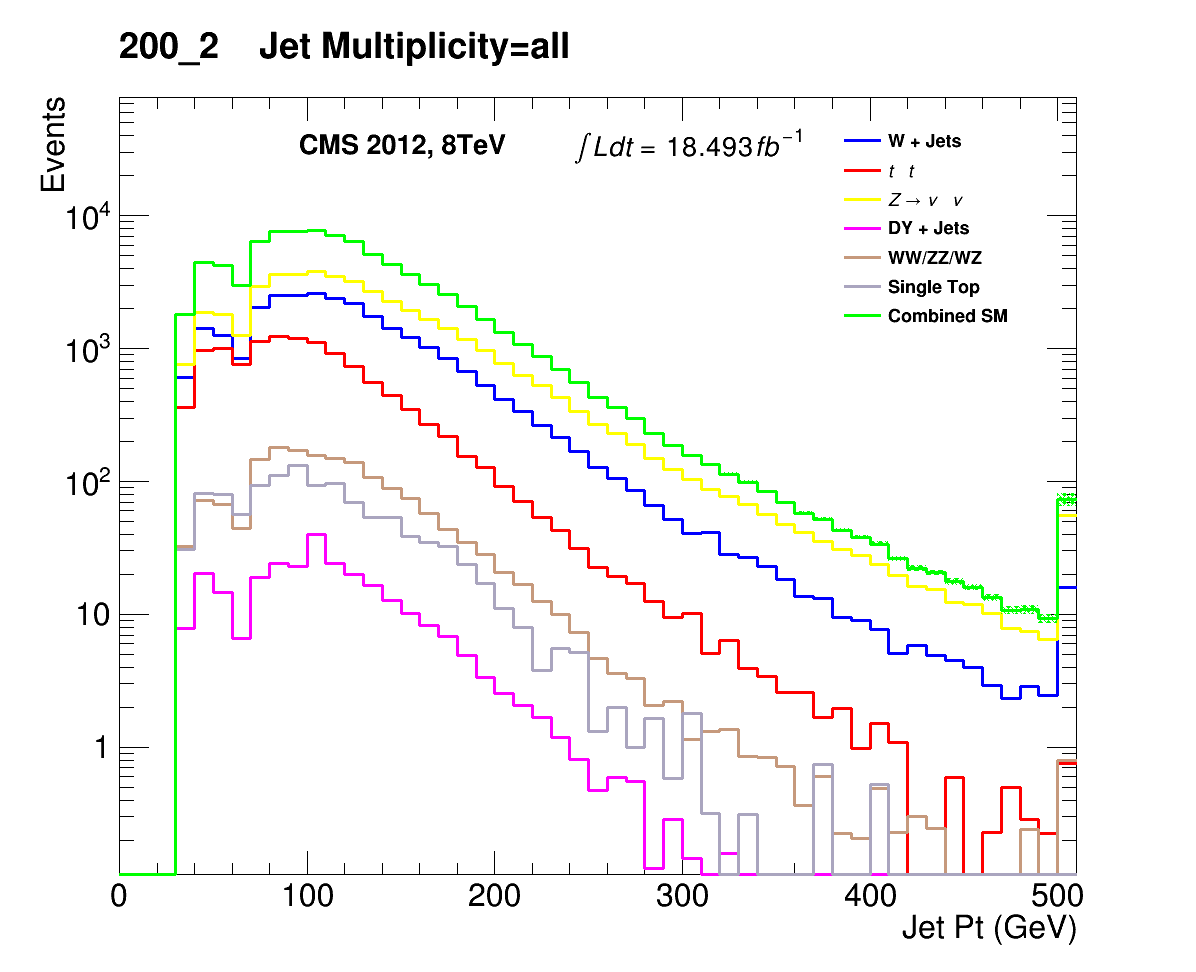
\includegraphics[width=\textwidth]{Figs/datamc/had/v1/CommonJetPt_all_200_upwards}
      \caption{Jet \Pt}
    \end{subfigure} \\
    \caption{\label{fig:datamc_had_inc}
    Kinematic distributions of all relevant simulated MC samples following
    the full hadronic signal selection. The 
    sum of the individual sample contributions is shown in green. Plots
    are for an inclusive selection of $\HT>200$~\gev, $\nj\geq2, \nb\geq0$.
    }
\end{figure}

% \begin{table}[ht!]
%   \caption{The cutflow of the hadronic selection in data. The subscript `fail'
%   indicates an object which did not meet all ID requirements, and so is not
%   considered as a `common object'. The event selection follows an inclusive
%   selection in data of $\HT > 375$~\gev, $\nj \geq 2$ and $\nb \geq 0$. }
%   \label{tab:had_data_cutflow}
%   \centering
%   \footnotesize
%   \begin{tabular}{ lcc }
%     \hline
%     \hline
%     Cut    & Eff (\%) & N \\
%     \hline
%   Event Count  & 100.00  & 161866108 \\
%   Good Event JSON Filter  & 94.97  & 153716716 \\
%   $\nj \geq 2$  & 98.68  & 151689664 \\
%   MET Filters & 98.81  & 149885013 \\
%   Vertex Noise Filter & 99.91  & 149746017 \\
%   DeadECAL Filter & 35.44  & 53066597 \\
%   Select seed Trigger & 3.76  & 1995549 \\
%   $n_{e} = 0$ & 98.48  & 1965269 \\
%   $n_{\gamma} = 0$  & 97.70  & 1920124 \\
%   $n_{\mu} = 0$ & 98.36  & 1888711 \\
%   $\text{EMF}_{max}$ for all jets > 0.1 & 99.99  & 1888576 \\
%   Leading jet \Pt > 100~\gev  & 97.83  & 1847501 \\
%   Leading jet $\eta$ < 2.5  & 97.31  & 1797777 \\
%   Sub-Leading jet \Pt > 100~\gev  & 81.75  & 1469654 \\
%   $n_{jet, fail} = 0$ & 81.73  & 1201096 \\
%   $\Delta R(\mu^i_{fail}, jet^j) < 0.5$ & 98.77  & 1186370 \\
%   $(\sum_{}^{n_{vertices}}{\Pt}$) / \HT & 100.00  & 1186368 \\
%   recHitCut & 98.44  & 1167861 \\
%   $n_{SIT} = 0$ & 85.77  & 1001646 \\
%   \mindphistar > 0.3  & 19.50  & 195361 \\
%   \HT > 375~\gev  & 73.33  & 143255 \\
%   \mhtmet < 1.25  & 9.26  & 13263 \\
%   \alphat > 0.55  & 38.25  & 5073 \\
%     \hline
%     \hline
%   \end{tabular}
% \end{table}

\begin{table}[ht!]
  \caption{The cutflow of the hadronic selection in data. The subscript `fail'
  indicates an object which did not meet all ID requirements, and so is not
  considered as a `common object'. The event selection follows an inclusive
  selection in data of $\HT > 375$~\gev, $\nj \geq 2$ and $\nb \geq 0$. }
  \label{tab:had_data_cutflow}
  \centering
  \footnotesize
  \begin{tabular}{ lcc }
    \hline
    \hline
    Cut Name    & Eff (\%) & N \\
    \hline
    Signal Trigger Accept  & 100.00  & 12843698.00 \\
    Good Event JSON Filter  & 95.32  & 12242217.00 \\
    $\nj \geq 2$  & 98.93  & 12110634.00 \\
    MET Filters & 98.68  & 11951541.00 \\
    Vertex Noise Filter & 99.92  & 11941983.00 \\
    DeadECAL Filter & 25.59  & 3056360.00 \\
    $n_{e} = 0$ & 98.62  & 3014305.00 \\
    $n_{\gamma} = 0$  & 97.82  & 2948741.00 \\
    $n_{\mu} = 0$ & 98.77  & 2912517.00 \\
    Leading jet \Pt > 100 \gev  & 98.20  & 2860068.00 \\
    Leading jet $\eta$ < 2.5  & 97.29  & 2782463.00 \\
    Sub-Leading jet \Pt > 100 \gev  & 84.24  & 2343910.00 \\
    $n_{j, fail} = 0$ & 83.45  & 1955899.00 \\
    $\Delta R(\mu^i_{fail}, jet^j) < 0.5$ & 98.87  & 1933858.00 \\
    $n_{SIT} = 0$ & 84.27 & 1629716.00 \\
    \HT > 375 \gev  & 93.45  & 1522986.00 \\
    \alphat > 0.55  & 0.55  & 8305.00 \\
    \mhtmet < 1.25  & 66.82  & 5549.00 \\
    \mindphistar > 0.3  & 90.83  & 5040.00 \\
    \hline
    \hline
  \end{tabular}
\end{table}




